\chapter{Παράλληλος Προγραμματισμός}

Οι εφαρμογές σήμερα, έχουν όλο και μεγαλύτερες απαιτήσεις σε υπολογιστική ισχύ. Η εγκυρότητα των μετεωρολογικών προβλέψεων, η ακρίβεια των αναλύσεων των δομικών κατασκευών των μηχανικών, η δημιουργία ρεαλιστικών γραφικών στους υπολογιστές, ο αριθμός των αεροπορικών κρατήσεων που επεξεργάζονται ανά δευτερόλεπτο και ο αριθμός των μεταφορών κεφαλαίων που επεξεργάζονται ανά δευτερόλεπτο βασίζονται στην ταχύτητα επεξεργασίας μεγάλου όγκου δεδομένων. Επιπλέον, η πρόοδος που έχει σημειωθεί τα τελευταία χρόνια στον τομέα της τεχνητής νοημοσύνης, όπως η εξέλιξη στους αλγόριθμους μηχανικής μάθησης, οφείλεται στην μεγαλύτερη ταχύτητα εκτέλεσης και τους πόρους που προσφέρουν οι σύγχρονες υπολογιστικές συσκευές.

Τις δεκαετίες του 1980 και 1990, η ταχύτητα των μικροεπεξεργαστών άρχισε να αυξάνεται με μεγάλο ρυθμό, λόγο της αύξησης της ταχύτητας του ρολογιού της κεντρικής μονάδας επεξεργασίας και τις βελτιώσεις στο σχεδιασμό υλικών (\en{hardware}). Όμως, αυτή η τάση σταμάτησε το 2003, λόγω της μεγάλης κατανάλωσης ενέργειας που προκύπτει από την αύξηση της συχνότητας του ρολογιού και ζητήματα απαγωγής θερμότητας. Λύση σε αυτό το πρόβλημα δόθηκε με τη χρήση πολλαπλών επεξεργαστικών πυρήνων σε ένα υπολογιστικό σύστημα. Με αυτό τον τρόπο είναι δυνατή η εκτέλεση πολλών εντολών παράλληλα κρατώντας την κατανάλωση ενέργειας χαμηλά.

Για την αξιοποίηση της υπολογιστικής ισχύς των πολλαπλών πυρήνων, χρειάστηκε να γίνει αλλαγή στο προγραμματιστικό μοντέλο που ακολουθούσαμε μέχρι σήμερα. Παραδοσιακά, τα προγράμματα αποτελούνται από μια ακολουθία εντολών που εκτελούνται από έναν επεξεργαστή σειριακά. Ο παράλληλος προγραμματισμός αναφέρεται στον διαμοιρασμό μιας εργασίας σε επιμέρους διεργασίες οι οποίες μπορούν να εκτελεστούν ταυτόχρονα από διαφορετικές επεξεργαστικές μονάδες, με στόχο τη μείωση στο χρόνο εκτέλεσης.

Τα στοιχεία για παράλληλη επεξεργασία που συναντάμε σε κάθε υπολογιστή είναι η \en{CPU} – κεντρική μονάδα επεξεργασίας, και η \en{GPU} – κάρτα γραφικών. Η \en{CPU} εκτελεί όλους τους υπολογισμούς και διαχειρίζεται όλες τις διεργασίες που είναι απαραίτητες για τη λειτουργία ενός λειτουργικού συστήματος. Περιλαμβάνει ένα περίπλοκο σχεδιασμό ελέγχου που επιτρέπει μεγάλη ευελιξία και απόδοση. Η \en{GPU}, αν και αρχικά σχεδιάστηκε για να μπορεί να εκτελεί πολλές ταυτόχρονες πράξεις για γραφικά, περιλαμβάνει πολλά επεξεργαστικά στοιχεία με πιο απλό σχεδιασμό ελέγχου και πλέον χρησιμοποιείται και για προγραμματισμό γενικού σκοπού. Τα δύο αυτά στοιχεία συνεργάζονται για την πιο γρήγορη επίλυση προβλημάτων. Συνδέοντας πολλά μηχανήματα με επεξεργαστικά στοιχεία σε κόμβους ή μέσω δικτύων, μπορούμε να δημιουργήσουμε συστοιχίες υπολογιστών (\en{cluster}) με πολύ μεγάλη υπολογιστική ισχύ. [21]

\section{Παράλληλος προγραμματισμός με \en{CPU}}
Τα σύγχρονα υπολογιστικά συστήματα διαθέτουν επεξεργαστές \en{CPU} με πολλαπλούς πυρήνες και υλικό που προσφέρεται για παραλληλία. Υπάρχουν τρείς τρόποι που μια \en{CPU} επιτρέπει την επιτάχυνση μέσω παραλληλίας: χρήση διανυσματικών επεξεργαστών (\en{vectorization}), πολλαπλοί πυρήνες και νήματα (\en{threading}), διαμοιρασμένη μνήμη.

\subsubsection{Διανυσματικοί επεξεργαστές – \en{vector processors}}

Η σύγχρονη αρχιτεκτονική επεξεργαστών περιλαμβάνει χαρακτηριστικά όπως διευρυμένους καταχωρητές (\en{wide registers}) και διευρυμένες επεξεργαστικές μονάδες (\en{wide processing units}) που επιτρέπουν την επεξεργασία κατά διανύσματα (\en{vector processing}), δηλαδή ταυτόχρονη επεξεργασία των τιμών ενός διανύσματος αντί για μία τιμή. Αυτή η μέθοδος είναι γνωστή ως \en{SIMD – Single Instruction Multiple Data}, όπου μία εντολή χρησιμοποιείται για την επεξεργασία πολλών δεδομένων. Για παράδειγμα, για τον υπολογισμό του αθροίσματος δύο διανυσμάτων:

\selectlanguage{english}
% \usemintedstyle{bw}
\begin{center}
\begin{minipage}{0.5\textwidth} 
\begin{minted}{text}
    for (i = 0; i < count; i++) 
      c[i] = a[i] + b[i]; 
    }
\end{minted}
\end{minipage}
\end{center}
  \selectlanguage{greek}

% Εικόνα 3.1 
\begin{Illustration}[!h] 
	\centering
	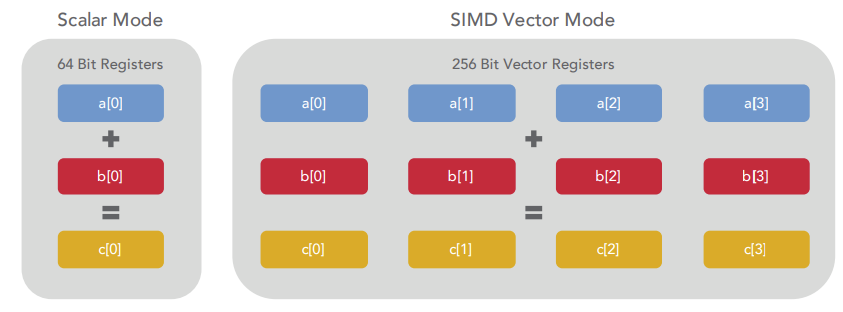
\includegraphics[width=\textwidth]{images/image043.png} 
	\caption{Πρόσθεση με χρήση διευρυμένους καταχωρητές 256\en{-bit} [22]}
	\label{image-registers-add}
\end{Illustration}

έστω ότι θέλουμε να υπολογίσουμε το άθροισμα αριθμών 64\en{-bit} διπλής ακρίβειας τύπου \src{float}. Αντί για το άθροισμα ενός ζεύγους αριθμών κάθε φορά, μπορούμε να χρησιμοποιήσουμε διευρυμένους καταχωρητές των 256\en{-bit} και να αθροίσουμε τέσσερα ζεύγη αριθμών ταυτόχρονα.
Ο πιο απλός τρόπος για την εφαρμογή της επεξεργασίας κατά διανύσματα είναι μέσω του μεταγλωττιστή (\en{compiler}) με την ενεργοποίηση των κατάλληλων επιλογών (\en{flags}). Στον \en{GCC compiler} προσθέτοντας τις επιλογές \src{-O3 ή -ftree-slp-vectorize, -ftree-vectorize,} μαζί με άλλες βελτιστοποιήσεις που πραγματοποιεί στον κώδικα, ο μεταγλωττιστής εντοπίζει τα τμήματα του κώδικα που θεωρεί ασφαλή για την εφαρμογή διανυσματικής επεξεργασίας. Με την επιλογή \src{-fopt-info-vec-optimized}, ο μεταγλωττιστής τυπώνει μηνύματα για τα τμήματα του κώδικα που έχουν υποστεί διανυσματική επεξεργασία. Αυτή η μέθοδος αποτελεί έναν γρήγορο και απλό τρόπο για βελτιστοποίηση της . Ωστόσο, ο μεταγλωττιστής δεν μπορεί πάντα να αναγνωρίσει όλα τα τμήματα του κώδικα που μπορούν να βελτιστοποιηθούν, καθώς μπορεί να χρειάζεται περισσότερες πληροφορίες.

Μπορούμε να δώσουμε περισσότερες πληροφορίες στον μεταγλωττιστή για τη δομή του κώδικα και να έχουμε καλύτερο έλεγχο της διανυσματοποίησης (\en{vectorization}) με εντολές τύπου \src{pragma}. Οι εντολές αυτές είναι για τον προεπεξεργαστή (\en{preprocessor}) και ξεκινάνε με τη δήλωση \src{\#pragma}. Τέτοιες εντολές παρέχει η \en{OpenMP}, στην οποία θα αναφερθούμε εκτενέστερα παρακάτω. Ένα απλό παράδειγμα φαίνεται εδώ:

\selectlanguage{english}
\begin{center}
\begin{minipage}{0.5\textwidth}
\begin{minted}{text}
    #pragma omp simd
    for (int n = 0; n < N; n++)
      a[n] += b[n];
\end{minted}
\end{minipage}
\end{center}
\selectlanguage{greek}

Οι εντολές τύπου \src{\#pragma} έχουν καλύτερη απόδοση σε σύγκριση με την απλή προσθήκη επιλογών βελτιστοποίησης (\en{flags}) στον μεταγλωττιστή, καθώς επιτρέπουν την εφαρμογή διανυσματικής επεξεργασίας ακόμα και σε περιπτώσεις περίπλοκων βρόχων.
Για ακόμη μεγαλύτερο έλεγχο στις \en{SIMD} πράξεις χρησιμοποιούμε εσωτερικές συναρτήσεις \en{(intrinsics) SSE (Streaming SIMD Extensions} – Επεκτάσεις \en{SIMD} συνεχούς ροής) και \en{AVX (Advanced Vector Extensions} – Προχωρημένες επεκτάσεις διανυσμάτων), τα οποία είναι δύο σύνολα εντολών που αναγνωρίζει ο μεταγλωττιστής και επιτρέπει τον ορισμό πράξεων σε χαμηλότερο επίπεδο.

Ένα παράδειγμα για το πώς φαίνεται ο κώδικας για πολλαπλασιασμό πίνακα με διάνυσμα υλοποιημένος με εσωτερικές συναρτήσεις φαίνεται παρακάτω:
 
\subsubsection{Πολλαπλοί πυρήνες και νήματα}

Οι σύγχρονοι επεξεργαστές διαθέτουν πάνω από έναν πυρήνα και κοινή μνήμη στην οποία όλοι οι πυρήνες έχουν πρόσβαση. Οι πολλαπλοί πυρήνες επιτρέπουν την εκτέλεση διεργασιών ταυτόχρονα ώστε να μειώνεται ο συνολικός χρόνος εκτέλεσης ενός προγράμματος. Το νήμα (\en{thread}), είναι μία ακολουθία εκτέλεσης εντολών μέσα σε μία διεργασία. Όλα τα νήματα που ανήκουν στην ίδια διεργασία έχουν πρόσβαση στα δεδομένα της διεργασίας σε κοινή μνήμη αλλά μπορούν να εκτελούνται παράλληλα.
 
% Εικόνα 3.2 
\begin{Illustration}[!h] 
	\centering
	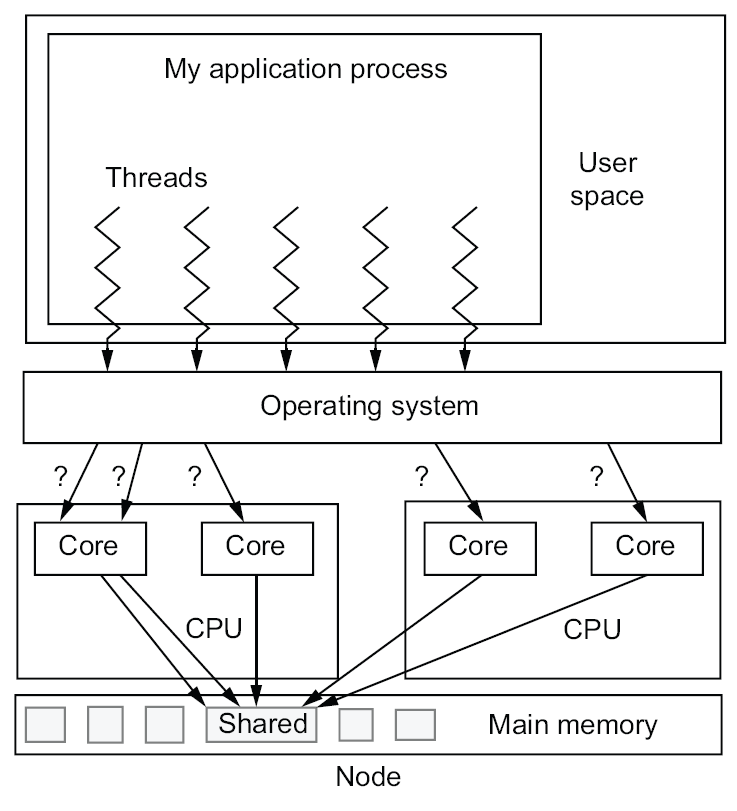
\includegraphics[width=0.45\textwidth]{images/image045.png} 
	\caption{Σύστημα πολλαπλών πυρήνων και κοινής μνήμης [23]}
	\label{image-multicore-shared-mem}
\end{Illustration}

\subsection{\en{OpenMP}}

To \en{OpenMP} χρησιμοποιείται για ανάπτυξη πολυνηματικών (\en{multithreaded}) παράλληλων εφαρμογών σε συστήματα κοινής μνήμης. Είναι ένα \en{API (Application Programming Interface} – Διεπαφή προγραμματισμού εφαρμογής) που επιτρέπει την εύκολη επεκτασιμότητα σειριακών προγραμμάτων γραμμένων σε \en{C,C++} ή \en{Fortran} σε παράλληλα με τη χρήση οδηγιών (\en{directives}) προς τον μεταγλωττιστή και μιας βιβλιοθήκης συναρτήσεων. Οι οδηγίες ορίζουν στο σειριακό πρόγραμμα περιοχές του κώδικα που μπορούν να εκτελεστούν παράλληλα και δίνουν πληροφορίες στον μεταγλωττιστή σχετικά με τις μεταβλητές και τον τρόπο διαμοιρασμού των επαναλήψεων ενός βρόχου στα διαθέσιμα νήματα. Δίνει έναν εύκολο και ευέλικτο τρόπο βελτιστοποίησης της ταχύτητας με παράλληλο προγραμματισμό. 
Ένα παράδειγμα κώδικα φαίνεται παρακάτω:

\selectlanguage{english}
\begin{center}
\begin{minipage}{0.5\textwidth}
\begin{minted}{text}
    #pragma omp parallel for
    for (int i = 0;i < N; i++)
        do_work(i);
\end{minted}
\end{minipage}
\end{center}
\selectlanguage{greek}

Οι οδηγίες του \en{OpenMP} ξεκινάνε με \src{\#pragma omp} και με το \src{parallel} δημιουργεί νήματα καθένα από τα οποία θα εκτελέσουν ένα αντίγραφο του κώδικα που βρίσκεται μέσα στο δομημένο μπλοκ. Με το for οι επαναλήψεις μοιράζονται μεταξύ των νημάτων. Στο τέλος του μπλοκ, τα νήματα συγχρονίζονται και αφού όλα τελειώσουν του υπολογισμούς τους, το πρόγραμμα συνεχίζει την εκτέλεση του. Στην περίπτωση που ο μεταγλωττιστής ή το μηχάνημα που διαθέτουμε δεν υποστηρίζει παραλληλία με \en{OpenMP}, αγνοούνται οι εντολές \src{\#pragma} και το πρόγραμμα τρέχει κανονικά με σειριακό τρόπο.

Το \en{OpenMP} διαθέτει πολλά στοιχεία για δημιουργία νημάτων, διαμοιρασμό της εργασίας, διαχείριση του περιβάλλοντος μεταβλητών και λειτουργίες συγχρονισμού των νημάτων. Τα τελευταία χρόνια έχουν προστεθεί και λειτουργίες για υποστήριξη παραλληλίας σε κάρτες γραφικών.

\subsection{Προγραμματισμός σε \en{GPU}}

Τα τελευταία χρόνια, οι κάρτες γραφικών χρησιμοποιούνται για προγραμματισμό γενικής χρήσης. Αρχικά, οι \en{GPU} σχεδιάστηκαν με σκοπό την επιτάχυνση υπολογισμών που έχουν να κάνουν με γραφικά. Γι’ αυτό το λόγο, διαθέτουν πολλούς απλούς επεξεργαστές που μπορούν να εκτελούν μαζικά αριθμητικές πράξεις. Σήμερα, οι προγραμματιστές εκμεταλλεύονται την αρχιτεκτονική των \en{GPU} για την επιτάχυνση επιστημονικών και άλλων εφαρμογών. 
Η διαφορά με τις \en{CPU} είναι πως οι \en{GPU} εστιάζουν στην διεκπεραιωτική ικανότητα εκτέλεσης (\en{throughput}) των παράλληλων εφαρμογών, ενώ οι \en{CPU} εστιάζουν στην γρήγορη ταχύτητα εκτέλεσης (\en{latency}) σειριακών προγραμμάτων. Σε σχέση με την \en{CPU}, η \en{GPU} διαθέτει πολλούς επεξεργαστές, απλούς, λιγότερο ισχυρούς και με πιο χαλαρό μοντέλο μνήμης ώστε περισσότερα δεδομένα να επεξεργάζονται ταυτόχρονα. Αυτό έχει και σαν αποτέλεσμα την χαμηλότερη κατανάλωση ενέργειας σε σχέση με τις \en{CPU} αλλά λιγότερο ευέλικτες προγραμματιστικά. 
 
% Εικόνα 3.3 
\begin{Illustration}[!h] 
	\centering
	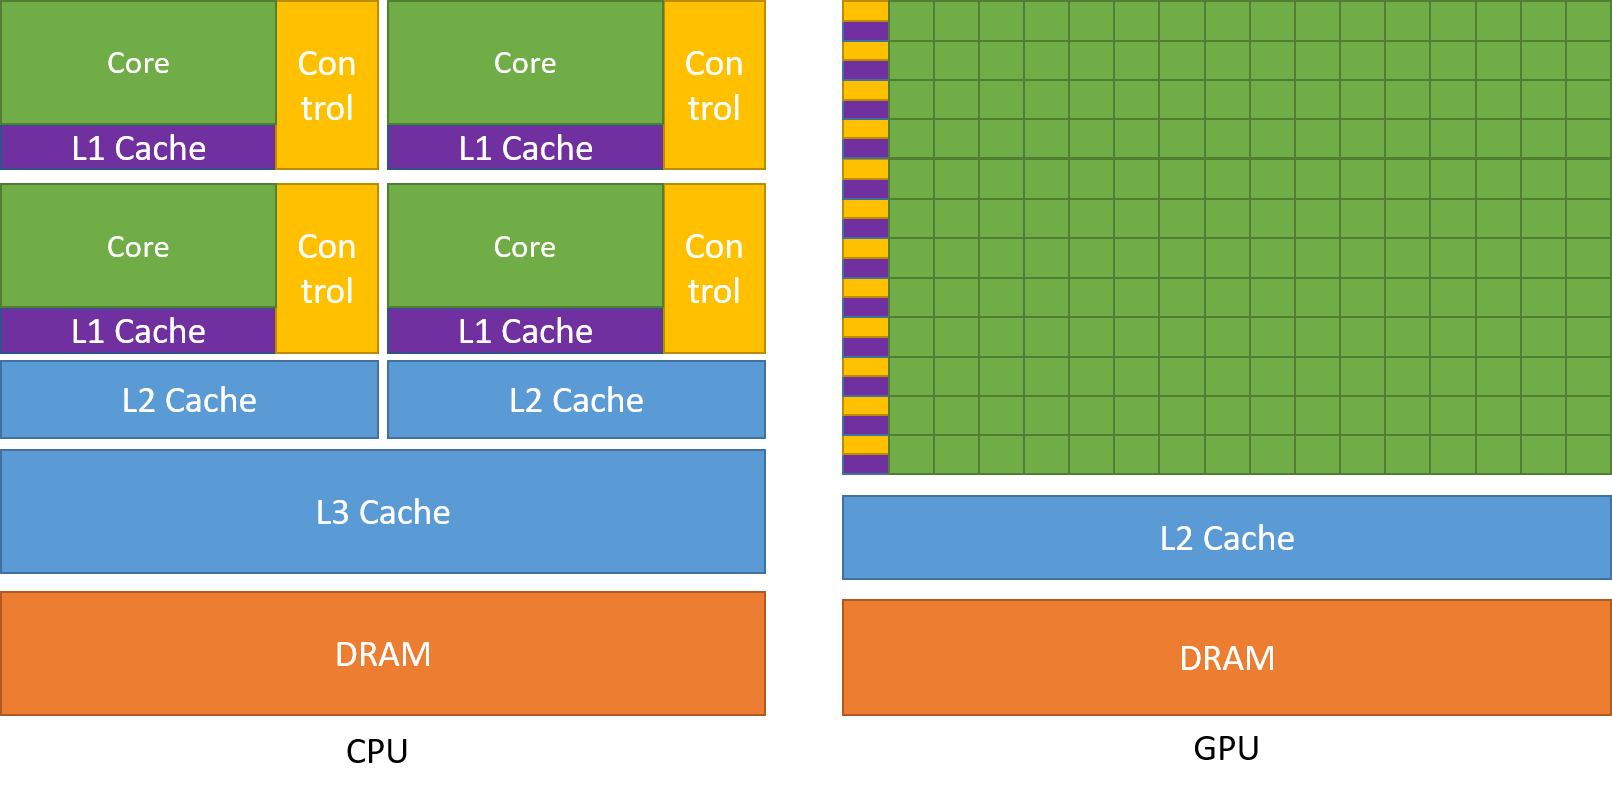
\includegraphics[width=0.8\textwidth]{images/image046.png} 
	\caption{Διαφορές αρχιτεκτονικής \en{CPU} και \en{GPU} [24]}
	\label{image-3.3}
\end{Illustration}

\subsection{\en{CUDA}}
Η \en{CUDA} είναι μια πλατφόρμα για παράλληλο προγραμματισμό και ένα προγραμματιστικό μοντέλο που αναπτύχθηκε από την \en{NVIDIA} για προγραμματισμό γενικού σκοπού σε κάρτες γραφικών \en{(GPGPU – General-Purpose Graphics Processing Unit).} Υποστηρίζει προγραμματισμό στις γλώσσες \en{C,C++, Fortran, Python} και \en{MATLAB} με επεκτάσεις σε αυτές για παράλληλο προγραμματισμό σε \en{GPU} της εταιρίας.

\subsection{Προγραμματιστικό Μοντέλο}

% Εικόνα 3.4 
\begin{Illustration}[!h] 
	\centering
	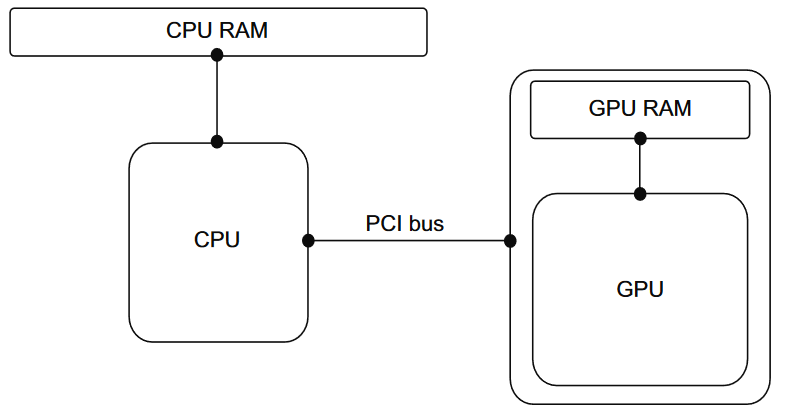
\includegraphics[width=0.75\textwidth]{images/image047.png} 
	\caption{Ετερογενές Σύστημα με \en{GPU} [23]}
	\label{image-3.4}
\end{Illustration}

Το προγραμματιστικό μοντέλο της \en{CUDA} αναφέρεται σε συστήματα ετερογενή, δηλαδή συστήματα που διαθέτουν δύο διαφορετικούς επεξεργαστές σε αυτά, την \en{CPU} και την \en{GPU}. Η \en{CPU} στην οποία τρέχει το κυρίως πρόγραμμα ονομάζεται κεντρικό σύστημα - \en{host} και η \en{GPU}, η οποία λειτουργεί βοηθητικά και θα εκτελέσει το υπολογιστικά βαρύ μέρος του κώδικα, ονομάζεται συσκευή - \en{device}. Η \en{GPU} λειτουργεί σαν συνεπεξεργαστής στο κεντρικό σύστημα, την \en{CPU}. Επίσης, η \en{CPU} και η \en{GPU} έχει η κάθε μία τη δική της ξεχωριστή μνήμη. 

Η \en{CPU} τρέχει το κυρίως πρόγραμμα και στέλνει εντολές στην \en{GPU} για το τι να κάνει. Είναι υπεύθυνη για την μεταφορά δεδομένων από και προς την \en{GPU}, την δέσμευση μνήμης στην \en{GPU} και την εκκίνηση συναρτήσεων που θα εκτελεστούν στην \en{GPU}.

Τα κομμάτια του κώδικα που θα εκτελεστούν στη συσκευή, στο κυρίως πρόγραμμα εμφανίζονται με τη μορφή συναρτήσεων και ονομάζονται πυρήνες (\en{kernels}). Όταν καλείται μια συνάρτηση πυρήνα, η συσκευή εκκινεί έναν μεγάλο αριθμό νημάτων που θα εκτελέσουν τον πυρήνα. Όλα τα νήματα που παράγει ένας πυρήνας σε μία κλήση συνολικά ονομάζονται πλέγμα (\en{grid}). Όταν ολοκληρωθεί η εκτέλεση όλων των νημάτων που ανήκουν στο ίδιο πλέγμα, η εκτέλεση του προγράμματος συνεχίζει στο κεντρικό σύστημα, μέχρι να συναντήσει τον επόμενο πυρήνα. [21]
 
% Εικόνα 3.5 
\begin{Illustration}[!h] 
	\centering
	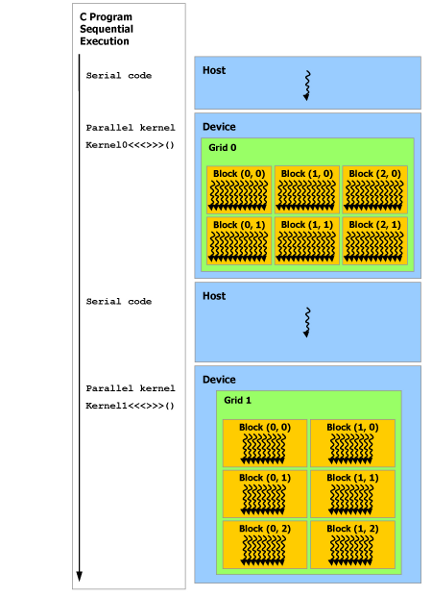
\includegraphics[width=0.5\textwidth]{images/image048.png} 
	\caption{Ροή εκτέλεσης προγράμματος σε ετερογενές σύστημα με \en{GPU} [24]}
	\label{image-3.5}
\end{Illustration}

Τα νήματα που ανήκουν σε ένα πλέγμα οργανώνονται σε μπλοκ (\en{block}). Όλα τα μπλοκ ενός πλέγματος έχουν τον ίδιο αριθμό νημάτων. Ο μέγιστος αριθμός νημάτων που μπορεί να έχει ένα μπλοκ εξαρτάται από την αρχιτεκτονική της κάρτας γραφικών, συνήθως είναι 1024.
 
% Εικόνα 3.6 
\begin{Illustration}[!h] 
	\centering
	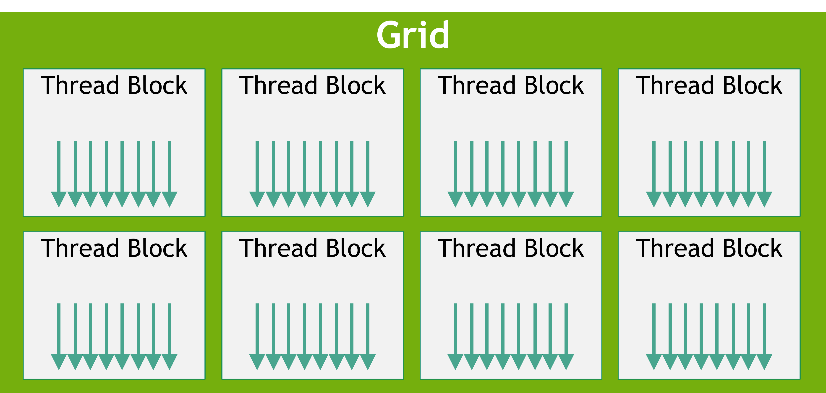
\includegraphics[width=0.7\textwidth]{images/image049.png} 
	\caption{Ένα πλέγμα από μπλοκ νημάτων [24]}
	\label{image-3.6}
\end{Illustration}

\subsubsection{Αρχιτεκτονική Κάρτας Γραφικών}
 
% Εικόνα 3.7 
\begin{Illustration}[!h] 
	\centering
	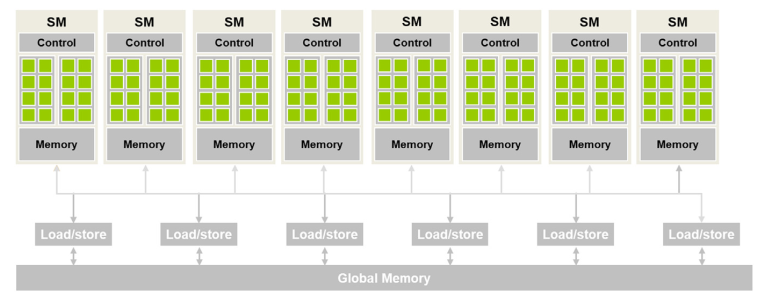
\includegraphics[width=\textwidth]{images/image050.png} 
	\caption{Αρχιτεκτονική Κάρτας Γραφικών [21]}
	\label{image-3.7}
\end{Illustration}


Αυτή η οργάνωση των νημάτων σε μπλοκ και πλέγματα προκύπτει από την αρχιτεκτονική της \en{GPU}. H \en{GPU} αποτελείται από πολυεπεξεργαστές συνεχούς ροής - \en{SM (streaming multiprocessors)} και κάθε \en{SM} διαθέτει πολλούς μικρούς επεξεργαστές που μπορούν να τρέχουν νήματα παράλληλα.

Όταν το σύστημα καλεί μια συνάρτηση πυρήνα εκκινείτε ένα πλέγμα από νήματα που θα εκτελέσουν τον κώδικα του πυρήνα. Η \en{GPU} αναλαμβάνει τον τρόπο διαμοιρασμού των μπλοκ νημάτων. Κάθε μπλοκ ανατίθεται σε ένα \en{SM}, ώστε τα νήματα που ανήκουν σε αυτό να εκτελεστούν παράλληλα. Η ανάθεση ενός μπλοκ σε ένα \en{SM} επιτρέπει στα νήματα που ανήκουν σε αυτό να αλληλεπιδρούν μεταξύ τους. Πολλά μπλοκ μπορούν να ανατεθούν στο ίδιο \en{SM}, όμως υπάρχει ένα όριο στο πόσα μπορούν να εκτελεστούν ταυτόχρονα.

Η \en{CUDA} δεν μπορεί να εγγυηθεί για τη σειρά και σε ποιο \en{SM} θα εκτελεστεί το κάθε μπλοκ. Αυτό δίνει το πλεονέκτημα στην \en{GPU} να είναι ευέλικτη και αποδοτική στην οργάνωση της εκτέλεσης των εργασιών. Επιπλέον, η εκτέλεση ενός προγράμματος \en{CUDA} είναι ανεξάρτητη του αριθμού των \en{SM} της συσκευής, πράγμα που σημαίνει πως το ίδιο πρόγραμμα μπορεί να τρέξει σε μια απλή συσκευή με ένα \en{SM}, αλλά και σε υπερυπολογιστή που διαθέτει πολλές \en{GPU}.

Όμως, δεν υπάρχει τρόπος να γνωρίζουμε σε ποιο \en{SM} θα εκτελεστεί το κάθε μπλοκ και δεν υπάρχει άμεσος τρόπος επικοινωνίας μεταξύ των μπλοκ. Εάν ένα μπλοκ περιμένει ένα άλλο για να ολοκληρωθεί, μπορεί να οδηγηθούμε σε αδιέξοδο (\en{dead lock}) εάν το δεύτερο μπλοκ έχει ολοκληρωθεί. Όλα τα νήματα που ανήκουν στο ίδιο μπλοκ πρέπει να ολοκληρωθούν ώστε να προγραμματιστεί η εκτέλεση του επόμενου μπλοκ στο \en{SM}.

\subsubsection{Μνήμη Κάρτας Γραφικών}
 
% Εικόνα 3.8 
\begin{Illustration}[!h] 
	\centering
	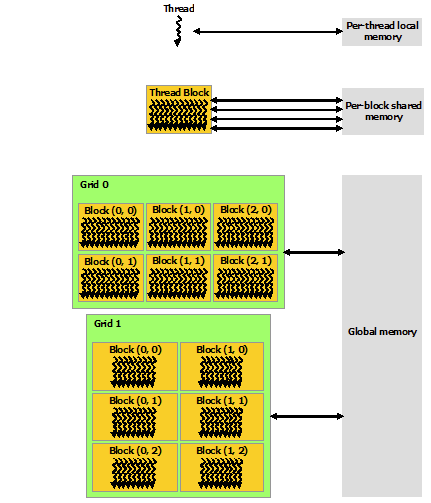
\includegraphics[width=0.65\textwidth]{images/image051.png} 
	\caption{Ιεραρχία μνήμης κάρτας γραφικών \en{CUDA} [24]}
	\label{image-3.8}
\end{Illustration}

Οι κάρτες γραφικών διαθέτουν τη δική τους μνήμη με δική της ιεραρχία. Κάθε νήμα έχει τοπική μνήμη (\en{local memory}), ιδιωτική για το νήμα. Κάθε μπλοκ από νήματα διαθέτει μια κοινή μνήμη (\en{shared memory}) στην οποία έχουν πρόσβαση όλα τα νήματα που ανήκουν σε αυτό. Είναι μνήμη που ανήκει στον \en{SM} και επιτρέπει την συνεργασία των νημάτων που ανήκουν στο ίδιο μπλοκ. Τέλος, υπάρχει και η καθολική μνήμη (\en{global memory}), από την οποία μπορούν να διαβάζουν και να γράφουν όλα τα νήματα οποιαδήποτε στιγμή. 

Η καθολική μνήμη είναι ο κύριος χώρος αποθήκευσης της κάρτας γραφικών και χρησιμοποιείται για την μεταφορά δεδομένων μεταξύ της \en{CPU} και της \en{GPU}. Ο προγραμματιστής χρειάζεται να δεσμεύσει χώρο στην καθολική μνήμη της συσκευής και να μεταφέρει δεδομένα από την μνήμη του κεντρικού συστήματος στην καθολική μνήμη της συσκευής. Μετά την εκτέλεση τον υπολογισμών στην συσκευή ο προγραμματιστής χρειάζεται να μεταφέρει τα αποτελέσματα πίσω στη μνήμη του κεντρικού συστήματος και να αποδεσμεύσει την μνήμη που δεν χρειάζεται πια από τη συσκευή. 

\subsubsection{Συγχρονισμός}

Τα νήματα έχουν πρόσβαση στα αποτελέσματα άλλων νημάτων μέσω της κοινής και της καθολικής μνήμης. Μπορούν να εργαστούν μαζί σε έναν υπολογισμό, αλλά με κάποιους περιορισμούς. Καθώς η \en{CUDA} δεν μπορεί να εγγυηθεί για την σειρά με την οποία θα εκτελεστούν τα νήματα, υπάρχει ο κίνδυνος ένα νήμα να διαβάσει ένα αποτέλεσμα πριν ένα άλλο νήμα υπολογίσει και γράψει το αποτέλεσμα αυτό.
 
% Εικόνα 3.9 
\begin{Illustration}[!h] 
	\centering
	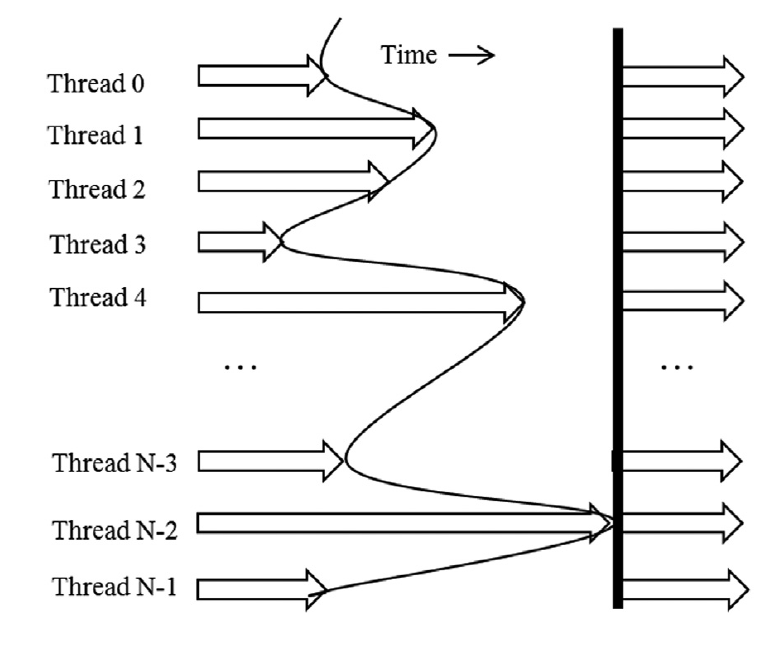
\includegraphics[width=0.5\textwidth]{images/image052.png} 
	\caption{Παράδειγμα συγχρονισμού των \en{threads} σε \en{barrier} [21]}
	\label{image-3.9}
\end{Illustration}


Η \en{CUDA} διαθέτει συναρτήσεις για συγχρονισμό των νημάτων. Ο πιο απλός τρόπος συγχρονισμού είναι το φράγμα (\en{barrier}). Το φράγμα είναι ένα σημείο στο πρόγραμμα όπου όλα τα νήματα σταματάνε και περιμένουν. Όταν όλα τα νήματα έχουν φτάσει στο φράγμα, μπορούν να συνεχίσουν την εκτέλεση του υπόλοιπου κώδικα.

\subsubsection{Πρόγραμμα σε \en{CUDA}}
Ένα τυπικό πρόγραμμα σε \en{CUDA} αποτελείται από την εξής ακολουθία εντολών:
\begin{enumerate}
\item Δήλωση μεταβλητών και δέσμευση μνήμης στο κεντρικό σύστημα και την συσκευή.
\item Αρχικοποίηση των δεδομένων στο κεντρικό σύστημα
\item Μεταφορά των δεδομένων από το κεντρικό σύστημα στη συσκευή
\item Εκτέλεση ενός ή περισσότερων πυρήνων
\item Μεταφορά των αποτελεσμάτων από την συσκευή στο κεντρικό σύστημα
\end{enumerate}

Ένα απλό πρόγραμμα \en{CUDA} που εκτελεί πρόσθεση δύο διανυσμάτων παράλληλα φαίνεται παρακάτω:
 
% Εικόνα 3.10
\begin{Illustration}[!h] 
	\centering
	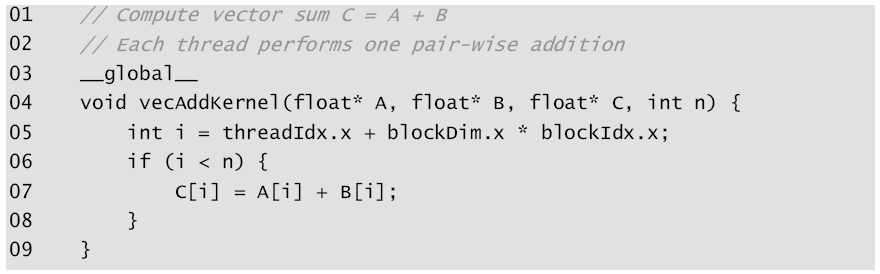
\includegraphics[width=0.6\textwidth]{images/image053.png} 
	\caption{Κώδικας συνάρτησης πυρήνα – \en{CUDA} [21]}
	\label{image-3.10}
\end{Illustration}


Με το \src{\_\_global\_\_} δηλώνεται η συνάρτηση πυρήνα που θα εκτελεστεί στη συσκευή.
Με την συνάρτηση \src{CUDAMalloc()} γίνεται η δέσμευση μνήμης στη συσκευή και στη συνέχεια με την \src{CUDAMemcpy()} αντιγράφονται οι τιμές των μεταβλητών. Η κλήση της συνάρτησης πυρήνα ακολουθείται από τα σύμβολα \mbox{\src{\en{< < <...> > >}}} με τα οποία δηλώνονται o αριθμός των νημάτων ανά μπλοκ και των μπλοκ στο πλέγμα που θα εκκινηθούν από τη συσκευή. Αφού εκτελεστεί ο πυρήνας, αντιγράφουμε τα αποτελέσματα από την συσκευή στο κεντρικό σύστημα με την \src{CUDAMemcpy()} και τέλος αποδεσμεύουμε την μνήμη της συσκευής για κάθε μεταβλητή με την \src{CUDAFree()}. 
 
% Εικόνα 3.11 
\begin{Illustration}[!h] 
	\centering
	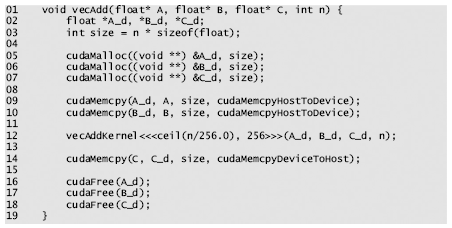
\includegraphics[width=0.6\textwidth]{images/image054.png} 
	\caption{Πάράδειγμα κώδικα σε \en{CUDA} [21]}
	\label{image-3.11}
\end{Illustration}

\subsection{\en{OpenCL}}

Μια άλλη επιλογή για παράλληλο προγραμματισμό ετερογενών συστημάτων είναι η \en{OpenCL}. Είναι ένα ανοικτό, δωρεάν πρότυπο για παράλληλο προγραμματισμό που υποστηρίζει κάρτες γραφικών όπως \en{NVIDIA} και \en{AMD} και σε πολλές άλλες συσκευές υλικού (\en{hardware}). Επιπλέον, είναι συμβατή με τους περισσότερους μεταγλωττιστές για \en{C} και \en{C++}. 

Η \en{OpenCL} είναι ένα αρκετά χαμηλού επιπέδου προγραμματιστικό μοντέλο με ευρεία αποδοχή, αλλά μακροσκελή (\en{verbose}) σύνταξη. Ένας από τους λόγους για τους οποίους η \en{OpenCL} θεωρείται ότι είναι μακροσκελής είναι ότι η επιλογή της συσκευής είναι αρκετά περίπλοκη. Ο προγραμματιστής πρέπει να εντοπίσει και να επιλέξει τη συσκευή στην οποία θα εκτελεστεί κάποια διεργασία και αυτό μπορεί να ανέλθει σε εκατοντάδες γραμμές κώδικα μόνο για να ξεκινήσει. 

Όπως και στην \en{CUDA} , έτσι και στην \en{OpenCL} ένα πρόγραμμα αποτελείται από δύο μέρη, τους πυρήνες που εκτελούνται στην συσκευή και το πρόγραμμα του κεντρικού συστήματος (\en{host}) που διαχειρίζεται την εκτέλεση των πυρήνων. Παρακάτω φαίνεται η αντιστοιχία της ορολογίας που χρησιμοποιεί η \en{OpenCL} με αυτή της \en{CUDA}.


\begin{table}[!h]
    \centering
    \selectlanguage{english}
    \begin{tabular}{ll}
        \textbf{OpenCL} & \textbf{CUDA} \\
        \hline
        NDRange & Grid \\
        Work Item & Thread \\
        Work Group & Block \\
        \hline
        Global Memory & Global Memory \\
        Local Memory & Shared Memory \\
        Private Memory & Local Memory \\
        Compute Unit & Streaming Multiproocessor \\
        Processing Element & Compute Core \\
        Work Item & Thread \\
        \hline
    \end{tabular}
    \selectlanguage{greek}
    \caption{Αντιστοιχεία \en{OpenCL} και \en{CUDA}}
    \label{tab:opencl-cuda}
\end{table}


Όπως αναφέρθηκε, η \en{OpenCL} μπορεί να υποστηρίξει πολλές διαφορετικές συσκευές υλικού, γι’ αυτό το λόγο έχει σύνθετο μοντέλο διαχείρισης των συσκευών. Η διαχείριση των συσκευών γίνεται με τον ορισμό του πλαισίου (\en{context}). Το πλαίσιο στην \en{OpenCL} είναι ο χώρος που περιλαμβάνει τις συσκευές, τη μνήμη για κάθε συσκευή και μια ουρά εντολών (\en{command queue}) ανά συσκευή. H ουρά εντολών είναι ο τρόπος που αλληλοεπιδρά το κεντρικό σύστημα με τις συσκευές για εκτέλεση πυρήνων, μεταφορές δεδομένων και λειτουργίες συγχρονισμού.
 
% Εικόνα 3.12 
\begin{Illustration}[!h] 
	\centering
	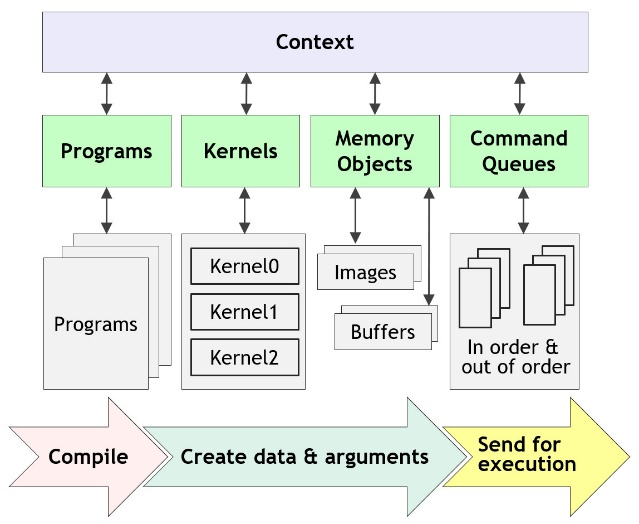
\includegraphics[width=0.5\textwidth]{images/image055.jpg} 
	\caption{Ακολουθία για εκτέλεση των πυρήνων στην \en{OpenCL} [25]}
	\label{image-3.12}
\end{Illustration}

Η \en{CUDA} εκτελεί αντίστοιχες διαδικασίες με την \en{OpenCL}, αλλά κρύβει την πολυπλοκότητα παρέχοντας τη δική της διεπαφή (\en{API}) για χρήση με συμβατές κάρτες γραφικών. 

\subsection{\en{OpenACC}}

Η \en{OpenACC} είναι ένα προγραμματιστικό μοντέλο, υψηλού επιπέδου, που βασίζεται σε οδηγίες προς τον μεταγλωττιστή (\en{directives}), σχεδιασμένο για \en{C/C++} και \en{Fortran} που δίνει λύση στην χρήση των \en{GPU} για επιτάχυνση υπολογισμών. Παρέχει μια απλοποιημένη προσέγγιση για τον προγραμματισμό ετερογενών αρχιτεκτονικών για υπολογιστική υψηλών επιδόσεων \en{(High-Performance Computing - HPC)}, επιτρέποντας στους προγραμματιστές να εισάγουν υποδείξεις στον κώδικά τους σχετικά με τον τρόπο που μπορεί να παραλληλοποιηθεί.

Το μοντέλο της \en{OpenACC} επιτρέπει στους επιστήμονες και τους προγραμματιστές να επικεντρωθούν στο επιστημονικό τους έργο χωρίς να χρειάζεται σε βάθος γνώση της αρχιτεκτονικής του υλικού (\en{hardware}), όπως για παράδειγμα στην \en{CUDA}. Οι προγραμματιστές μπορούν απλώς να εισάγουν οδηγίες στον κώδικά τους και ο μεταγλωττιστής αναλαμβάνει την παραλληλοποίηση και βελτιστοποίηση του κώδικα για την πλατφόρμα που έχει επιλεχθεί.

Το πλεονέκτημα του προγραμματισμού με οδηγίες είναι πως ο μεταγλωττιστής μπορεί να αγνοήσει τις οδηγίες και ο κώδικας να τρέξει σειριακά παράγοντας σωστά αποτελέσματα. Αυτό επιτρέπει τη διατήρηση μιας ενιαίας βάσης κώδικα, και επιπλέον, προσφέρει φορητότητα σε διαφορετικές πλατφόρμες. Η \en{OpenACC} χρησιμοποιείται κυρίως για παράλληλο προγραμματισμό σε κάρτες γραφικών, αλλά υποστηρίζει και άλλες αρχιτεκτονικές πολυπύρηνων επεξεργαστών. Μέχρι σήμερα, οι πλατφόρμες που υποστηρίζουν \en{OpenACC} περιλαμβάνουν τις αρχιτεκτονικές \en{x86} και \en{x64}, τις κάρτες γραφικών της \en{NVIDIA} και της \en{AMD}, επεξεργαστές \en{OpenPOWER, Knights Landing} και \en{ARM}. [26]

\subsubsection{Σύνταξη \en{OpenACC}}

Το \en{OpenACC} αποτελείται ένα σύνολο οδηγιών (\en{directives}) προς τον μεταγλωττιστή, βιβλιοθήκης συναρτήσεων και μεταβλητών περιβάλλοντος που επιτρέπει στον προγραμματιστή να εκφράσει τον παραλληλισμό που ενυπάρχει στον κώδικά, ώστε ο μεταγλωττιστής να μπορεί να τον μεταφράσει σε μορφή που να ταιριάζει σε διάφορες παράλληλες αρχιτεκτονικές.

Η σύνταξη των \textit{οδηγιών} προς τον μεταγλωττιστή σε \en{C/C++} έχει την παρακάτω μορφή:

\medskip
\src{\#pragma acc <directive> [clause [[,] clause] . . .] new-line}
\medskip

Η εντολές προς τον μεταγλωττιστή ξεκινούν με \src{\#pragma}, όπως ακριβώς και στην \en{OpenMP}. Το \src{acc} δηλώνει ότι αναφερόμαστε στην \en{OpenACC} και ακολουθείται από κάποιο \src{directive} το οποίο δίνει οδηγίες στον μεταγλωττιστή για το μπλοκ κώδικα που ακολουθεί. Το \en{clause} που είναι \textit{φράσεις} που παραμετροποιούν τη λειτουργία των \textit{οδηγιών}. 

Όπως σε κάθε γλώσσα προγραμματισμού για \en{GPU}, έτσι και στην \en{OpenACC}, υπάρχουν διάφορα στοιχεία που πρέπει να υπάρχουν και να εκτελούν τις εξής λειτουργίες:

\begin{enumerate}
\item Έκφραση των υπολογιστικών βρόχων σε παράλληλη μορφή για την \en{GPU}.
\item Μετακίνηση δεδομένων μεταξύ του κεντρικού συστήματος και της συσκευής
\item Λειτουργίες συγχρονισμού των νημάτων.
\end{enumerate}

Αυτά στην \en{OpenACC} υλοποιούνται με τις \textit{οδηγίες} που διαθέτει.

\subsubsection{Παραλληλοποίηση Κώδικα}

Το πιο βασικό στην \en{OpenACC} είναι ο διαμοιρασμός της εργασίας στα παράλληλα νήματα ώστε να επιτευχθεί καλύτερη απόδοση και να μειωθεί ο χρόνος εκτέλεσης. Η \en{OpenACC} διαμοιράζει τους βρόχους των επαναλήψεων σε νήματα αναθέτοντας μία επανάληψη ανά νήμα. Οι \textit{οδηγίες} που το κάνουν αυτό είναι το \src{kernels} και το \src{parallel}. 

Η \textit{οδηγία} \src{kernels}, δίνει εντολή στον μεταγλωττιστή να εντοπίσει τους βρόχους που μπορούν να εκτελεστούν παράλληλα στον κώδικα που βρίσκεται στο μπλοκ. Ο προγραμματιστής αφήνει τον μεταγλωττιστή να αναλύσει τον κώδικα και να παραλληλίσει τους βρόχους που θεωρεί πως είναι ασφαλές να το κάνει. Εάν θεωρήσει πως δεν μπορεί να παραλληλοποιηθεί, ο κώδικας θα τρέξει σειριακά. Και στις δύο περιπτώσεις ο μεταγλωττιστής εξασφαλίζει τα σωστά αποτελέσματα.

\selectlanguage{english}
\begin{center}
\begin{minipage}{0.5\textwidth}
\begin{minted}{text}
    #pragma acc kernels
    {
        for (int i = 0; i < N; i++) {
          c[i] = a[i] + b[i];
        }
        for (int i = 0; i < N; i++) {
          d[i] = a[i] + 5;
        }
    }
\end{minted}
\end{minipage}
\end{center}
\selectlanguage{greek}

Με την \textit{οδηγία} \src{parallel}, ο προγραμματιστής ενημερώνει τον μεταγλωττιστή ότι ο κώδικας μπορεί να παραλληλιστεί. Ο μεταγλωττιστής δημιουργεί \textit{ομάδες εργασίας} (\en{gangs}) στη συσκευή και κάθε ομάδα εργασίας θα εκτελέσει ολόκληρο το βρόχο που ακολουθεί. Οι \textit{ομάδες εργασίας}, είναι ομάδες από νήματα που ανήκουν σε \textit{μονάδες εργασίας} (\en{worker threads}) που εκτελούνται ανεξάρτητα, τα οποία αναλύονται παρακάτω. Για να διαμοιραστούν οι επαναλήψεις του βρόχου σε νήματα που θα εκτελεστούν παράλληλα, χρειάζεται η \textit{οδηγία} \src{loop}. 
 
% Εικόνα 3.13 
\begin{Illustration}[!h] 
	\centering
	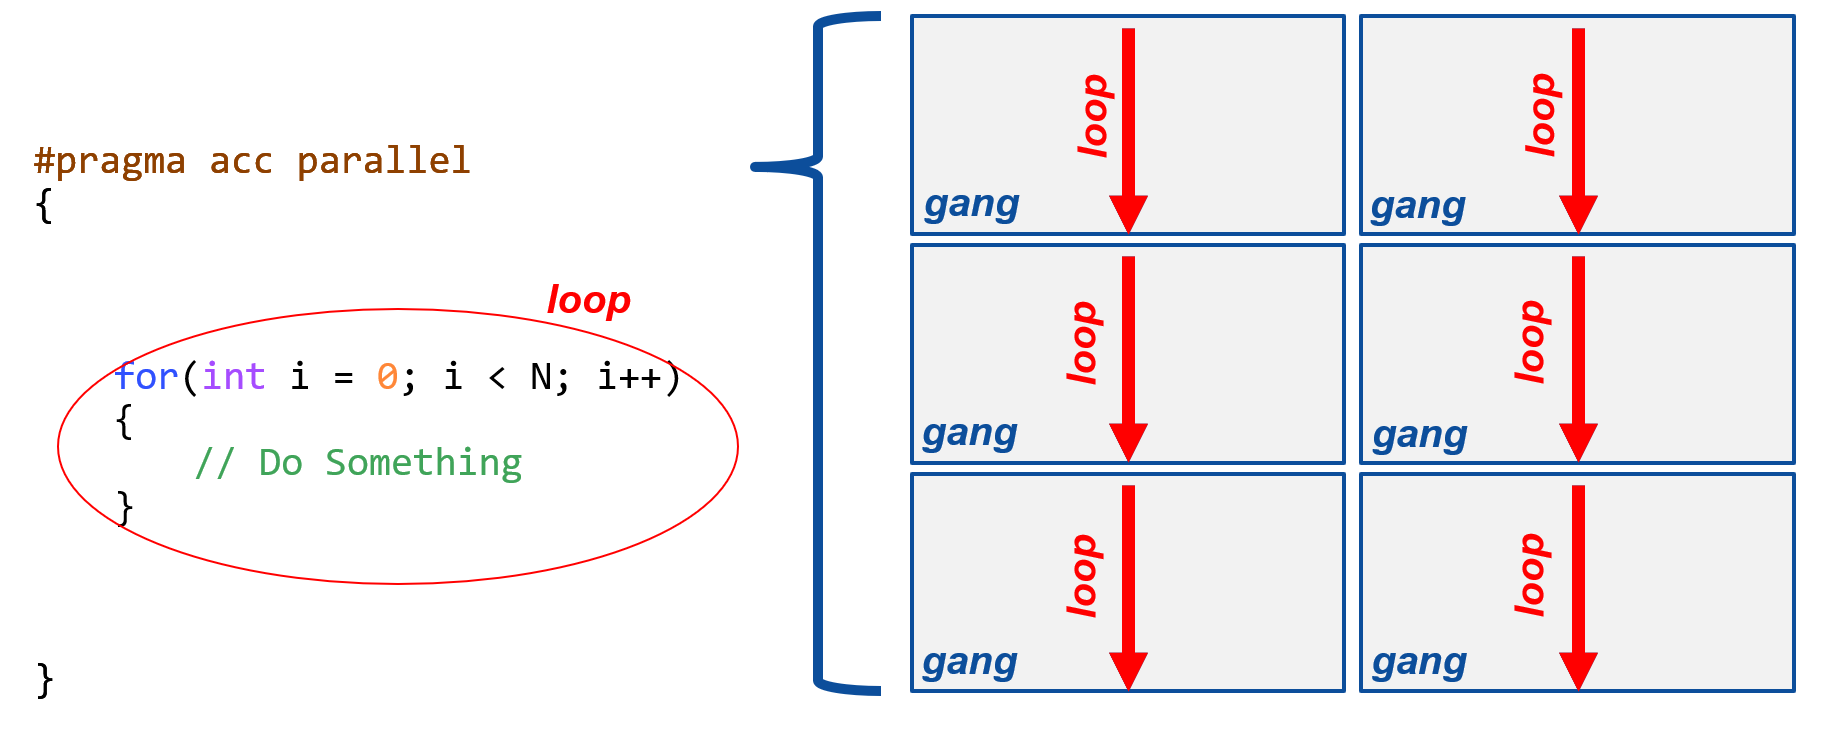
\includegraphics[width=0.7\textwidth]{images/image056.png} 
	\caption{ο βρόχος (\en{loop}) εκτελείται από όλες της ομάδες εργασίας (\en{gang}) [27]}
	\label{image-3.13}
\end{Illustration}

 
% Εικόνα 3.14 
\begin{Illustration}[!h] 
	\centering
	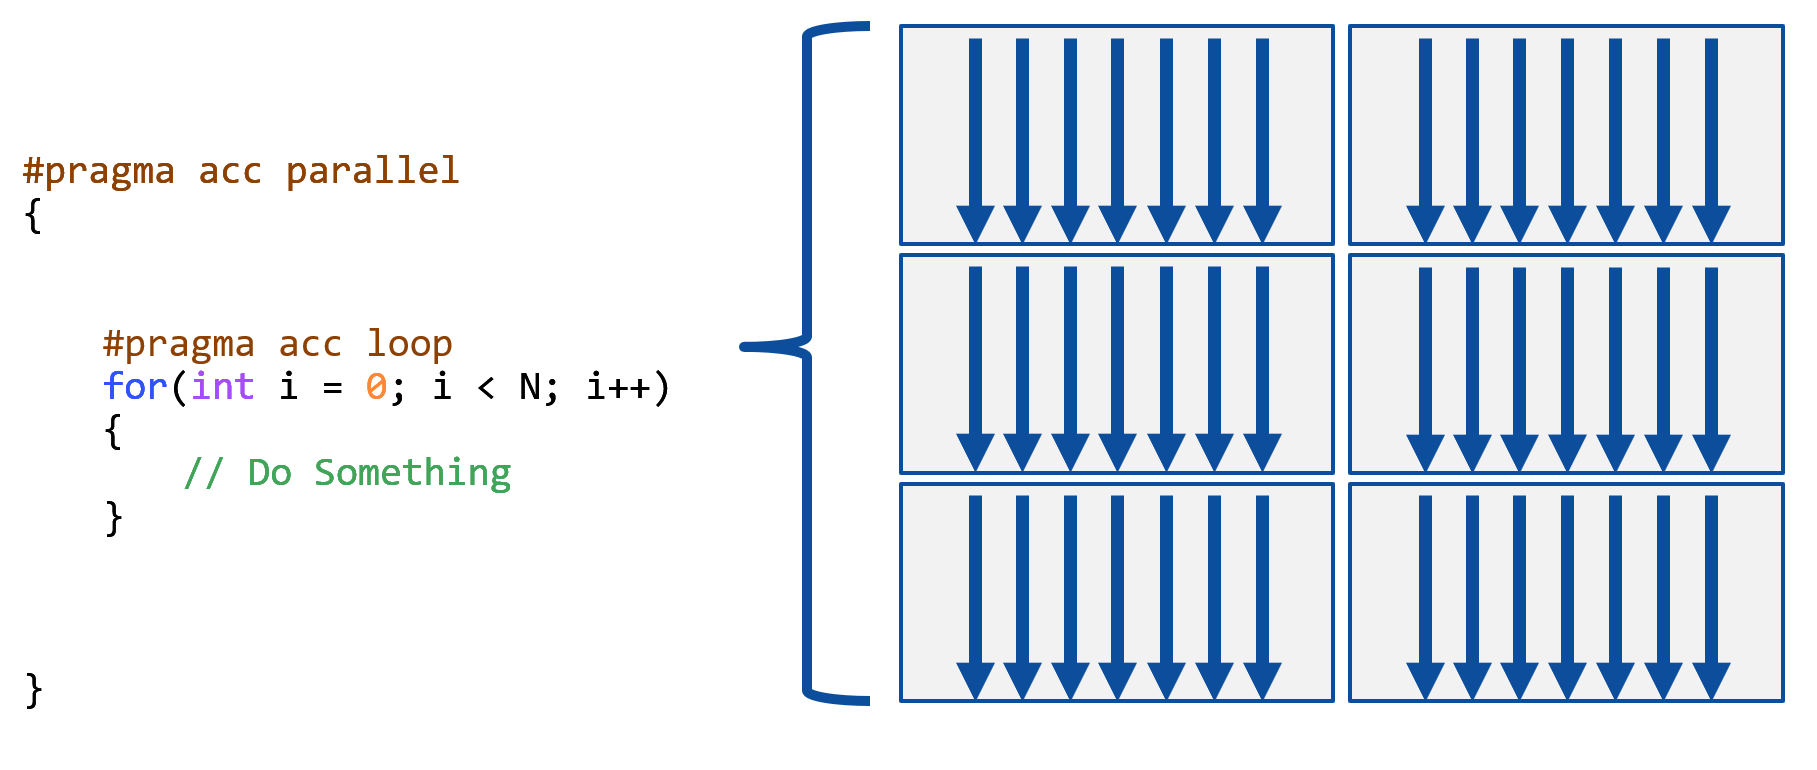
\includegraphics[width=0.7\textwidth]{images/image057.png} 
	\caption{με τη χρήση του \src{loop} οι επαναλήψεις διαμοιράζονται στις ομάδες εργασίας (\en{gang}) [27]}
	\label{image-3.14}
\end{Illustration}


Οι δύο \textit{οδηγίες} χρησιμοποιούνται συνδυαστικά και αναφέρονται στο βρόχο που ακολουθεί την εντολή \src{\#pragma}. Καθώς τον έλεγχο για την παραλληλοποίηση του κώδικα την έχει ο προγραμματιστής, θέλει προσοχή καθώς πιθανές εξαρτήσεις μεταξύ των δεδομένων στις επαναλήψεις μπορεί να οδηγήσουν σε λάθος αποτελέσματα.
  
\selectlanguage{english}
\begin{center}
\begin{minipage}{0.5\textwidth}
\begin{minted}{text}
    #pragma acc parallel loop
        for (int i = 0; i < N; i++) {
          c[i] = a[i] + b[i];
        }
    #pragma acc parallel loop
        for (int i = 0; i < N; i++) {
          d[i] = a[i] + 5;
        }
\end{minted}
\end{minipage}
\end{center}
\selectlanguage{greek}

Επιπλέον, το \src{loop} μπορεί να χρησιμοποιηθεί μέσα σε περιοχή που ορίζεται από την \textit{οδηγία} \src{kernels} σε περιπτώσεις που ο μεταγλωττιστής δεν μπορεί να αποφασίσει εάν είναι ανεξάρτητες οι επαναλήψεις μεταξύ τους.

\bigskip
\textbf{\textit{Υποβίβαση - \en{Reduction}}}
\medskip

Μία ειδική κατηγορία αλγορίθμων την οποία ο μεταγλωττιστής συνήθως δεν θα μπορέσει να παραλληλοποιήσει, είναι όταν μια μεταβλητή ή ένας πίνακας ενημερώνεται κατά τη διάρκεια κάθε επανάληψης ενός βρόχου. Ένα παράδειγμα τέτοιων αλγορίθμων είναι η εύρεση μέγιστου ή ελάχιστου ή ο υπολογισμός συνολικού αθροίσματος. Στον παράλληλο προγραμματισμό, οι πράξεις αυτές ονομάζονται \textit{πράξεις υποβίβασης} (\en{reduction}). Στην πράξη, αυτό που γίνεται είναι ότι ορίζεται μία μεταβλητή όπου το κάθε νήμα κάνει υπολογισμούς τοπικά, και στη συνέχεια ακολουθεί μία τελική πράξη που θα συνδυάσει όλες τις τοπικές μεταβλητές σε μία. 

Στην \en{OpenACC}, αυτό υλοποιείται με την \textit{φράση} \en{reduction} και χρησιμοποιείται ως εξής: 

\selectlanguage{english}
\begin{center}
\begin{minipage}{0.5\textwidth}
\begin{minted}{text}
        total = 0;
    #pragma acc parallel loop reduction(+ : total)
        for (i = 0; i < 100; i++) {
            total = total + data[i];
        }
\end{minted}
\end{minipage}
\end{center}
\selectlanguage{greek}

\subsubsection{Περιβάλλον Μεταβλητών}
 
% Εικόνα 3.15 
\begin{Illustration}[!h] 
	\centering
	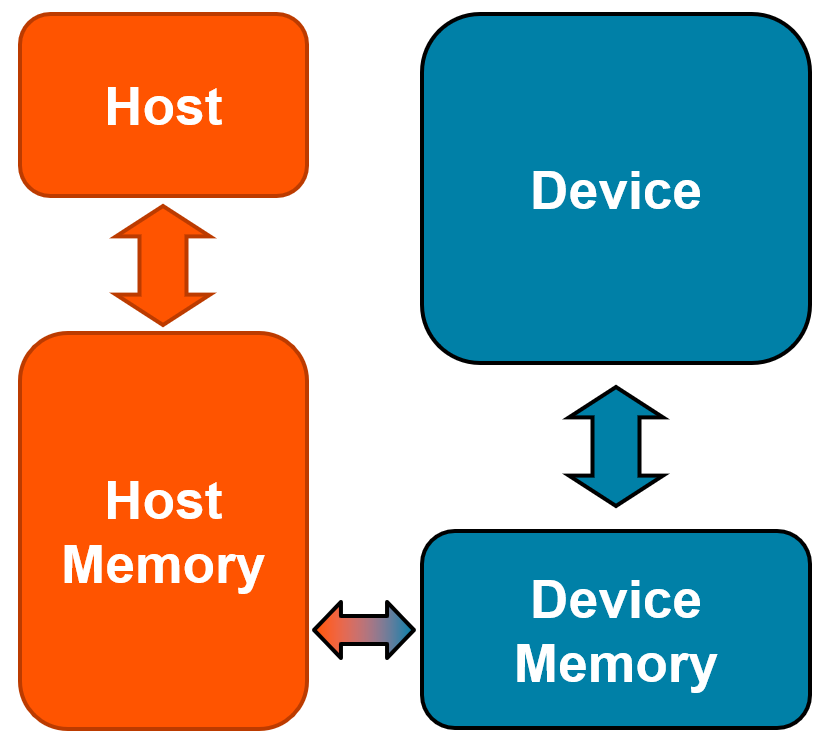
\includegraphics[width=0.5\textwidth]{images/image058.png} 
	\caption{Μοντέλο ετερογενούς συστήματος κεντρικού συστήματος (\en{host}) – συσκευής (\en{device}) [27]}
	\label{image-3.15}
\end{Illustration}


H \en{OpenACC} είναι σχεδιασμένη για ετερογενή συστήματα στα οποία η μνήμη της συσκευής που χρησιμοποιείται για την επιτάχυνση είναι ξεχωριστή από τη μνήμη του κεντρικού συστήματος, όπου τρέχει το κυρίως πρόγραμμα. Γι’ αυτό το λόγο είναι απαραίτητη η μεταφορά δεδομένων μεταξύ του κεντρικού συστήματος και της συσκευής. Στο μοντέλο της \en{OpenACC}, οι μεταφορές των δεδομένων γίνονται αυτόματα από τον μεταγλωττιστή, σε αντίθεση με τις γλώσσες χαμηλού επιπέδου, όπως η \en{CUDA}, όπου οι εντολές για δέσμευση μνήμης και μεταφοράς δεδομένων καταλαμβάνουν μεγάλο μέρος του κώδικα. 

Ωστόσο, ο μεταγλωττιστής για να εξασφαλίσει την σωστή λειτουργία του κώδικα, μπορεί να πραγματοποιεί περιττές μεταφορές δεδομένων από και προς τη μνήμη. Ο προγραμματιστής εισάγοντας τις κατάλληλες οδηγίες δίνει τις κατάλληλες πληροφορίες. Η εισαγωγή \textit{οδηγιών} για μεταφορά δεδομένων θεωρείται βελτιστοποίηση και πραγματοποιείται αφού έχουμε παραλληλοποιήσει τον κώδικα. 

Μερικές χαρακτηριστικές λειτουργίες που μπορεί να υποστηρίξει η \en{OpenACC} με χρήση \textit{φράσεων} (\en{clauses}) είναι: 

\begin{itemize}
\item \src{copy} – δεσμεύει μνήμη στη συσκευή για τις σχετικές μεταβλητές, αντιγράφει το περιεχομένων των μεταβλητών στη συσκευή, και αντιγράφει τα αποτελέσματα στο κεντρικό σύστημα στο τέλος της περιοχής.
\item \src{copyin} – έχει την ίδια λειτουργία με το \src{copy} με τη διαφορά πως στο τέλος της περιοχής δεν αντιγράφει το περιεχόμενο των μεταβλητών στο κεντρικό σύστημα.
\item \src{copyout} – ίδια λειτουργία με το \src{copy} με τη διαφορά πως δημιουργεί τις μεταβλητές χωρίς να τις αρχικοποιήσει, αντιγράφει μόνο τα αποτελέσματα στο τέλος από τη συσκευή στο κεντρικό σύστημα.
\item \src{create} – δεσμεύει χώρο στη συσκευή για τις σχετικές μεταβλητές, και απελευθερώνει τον χώρο στο τέλος της περιοχής, αλλά δεν αντιγράφει δεδομένα από και προς τη συσκευή.
\item \src{present} – δηλώνει πως οι μεταβλητές υπάρχουν στην συσκευή και δεν χρειάζεται γίνει κάποια ενέργεια. [28]
\end{itemize}

Η χρήση των παραπάνω \textit{φράσεων} συνδυάζεται με της \textit{οδηγίες} \src{parallel} και \src{kernels} που ορίζουν περιοχές παραλληλίας, αλλά και με την \textit{οδηγία} \src{data}, με το οποίο ο χρήστης ορίζει \textit{περιοχές δεδομένων} (\en{data regions}) που ορίζουν την \textit{διάρκεια ζωής των δεδομένων} (\en{data lifetime}) στην συσκευή.

\selectlanguage{english}
\begin{center}
\begin{minipage}{0.5\textwidth}
\begin{minted}{text}
    #pragma acc data create(x[0:N]) copyout(y[0:N])
    {
    #pragma acc parallel loop
    for (i = 0; i < N; i++) {
      y[i] = 0.0f;
      x[i] = (float)(i + 1);
    }
    
    #pragma acc parallel loop
    for (i = 0; i < N; i++) {
      y[i] = 2.0f * x[i] + y[i];
    }
    }
\end{minted}
\end{minipage}
\end{center}
  \selectlanguage{greek}


\subsection{Επίπεδα παραλληλισμού}

Για να εξασφαλίσει τη φορητότητα σε διαφορετικές αρχιτεκτονικές, η \en{OpenACC} ορίζει ένα αφαιρετικό μοντέλο για την απεικόνιση των πολλαπλών επιπέδων παραλληλισμού που μπορεί να διαθέτει ένας επεξεργαστής. Διακρίνονται τρία επίπεδα παραλληλίας: \textit{ομάδα εργασίας} - \en{gang}, \textit{μονάδα εργασίας} ή \textit{εργάτης} - \en{worker} και \textit{διάνυσμα} - \en{vector}. 
 
% Εικόνα 3.16 
\begin{Illustration}[!h] 
	\centering
	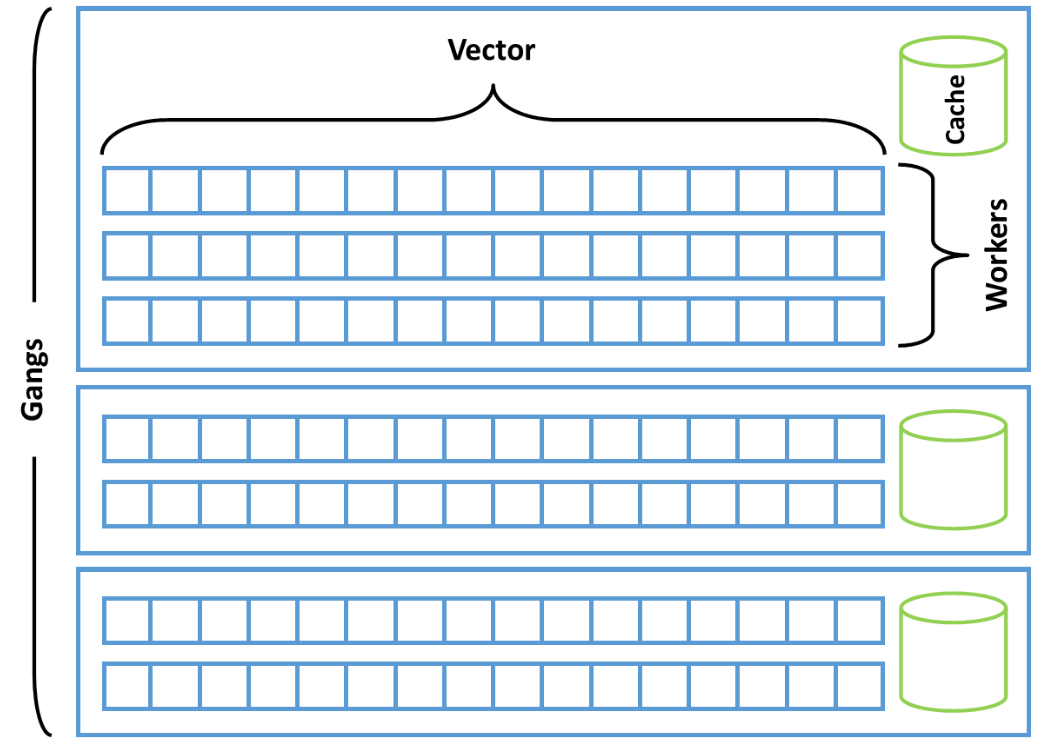
\includegraphics[width=0.6\textwidth]{images/image059.png} 
	\caption{Επίπεδα παραλληλισμού της \en{OpenACC} [28]}
	\label{image-3.16}
\end{Illustration}


Το \textit{διάνυσμα} (\en{vector}) είναι το χαμηλότερο επίπεδο παραλληλίας και αναφέρεται στην εκτέλεση της ίδιας εντολής σε διαφορετικά δεδομένα – \en{SIMD (Single instruction, Multiple Data} – μια εντολή, πολλά δεδομένα) για τις \en{CPU} ή \en{SIMT (Single Instruction, Multiple Threads} – μία εντολή, πολλά νήματα) στις \en{GPU}. Το μήκος του διανύσματος – \en{vector length} δηλώνει σε πόσα στοιχεία δεδομένων θα εκτελεστεί η ίδια εντολή. Η \textit{ομάδα εργασίας} (\en{gang}) είναι το υψηλότερο επίπεδο παραλληλίας, όπου κάθε \textit{ομάδα} εκτελείται ανεξάρτητα από τις άλλες και δε συγχρονίζονται μεταξύ τους. Η \textit{μονάδα εργασίας }ή\textit{ εργάτης} (\en{worker}) είναι ανάμεσα στα δύο επίπεδα. Μία \textit{ομάδα εργασίας} αποτελείται από έναν ή περισσότερους \textit{εργάτες}, οι οποίοι λειτουργούν σε ένα διάνυσμα κάποιου μήκους. Οι \textit{εργάτες} και τα διάνυσμα που ανήκουν στην ίδια \textit{ομάδα} έχουν πρόσβαση σε μία κοινή κρυφή μνήμη (\en{cache}) και επιτρέπεται ο συγχρονισμός μεταξύ τους.[28]

Για βελτιστοποίηση στον τρόπο αντιστοίχισης στο διαθέσιμο υλικό, η \en{OpenACC} διαθέτει φράσεις (\en{clauses}) για διαμοιρασμό της εργασίας. Μερικά ενδεικτικά είναι\src{ seq, auto, gang, worker, vector, tile, num\_gangs, num\_workers,} και \src{vector\_length}. [26]
